\documentclass[tikz,border=2pt]{standalone}
\usepackage{amsmath,amssymb}
\usepackage{pgfplots}
\pgfplotsset{compat=1.18}
\usetikzlibrary{arrows.meta}
\begin{document}
% CDF of a loss that is 0 with probability 0.8 and otherwise uniform on (0,100):
% a jump of 0.8 at the atom x = 0, then slope f_c = 0.002 up to F_X(100) = 1.
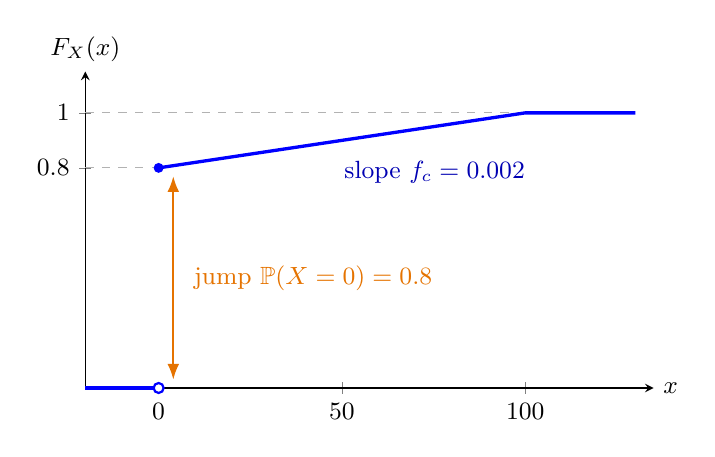
\begin{tikzpicture}[font=\small, >={Latex[length=2mm]}]
  \begin{axis}[
    axis lines=left, xmin=-20, xmax=135, ymin=0, ymax=1.15,
    xtick={0,50,100}, ytick={0.8,1},
    xlabel={$x$}, ylabel={$F_X(x)$},
    xlabel style={at={(axis description cs:1,0)}, anchor=west},
    ylabel style={rotate=-90, at={(axis description cs:0,1)}, anchor=south},
    width=8.8cm, height=5.6cm, clip=false]
    \draw[gray!60, thin, dashed] (axis cs:-20,0.8) -- (axis cs:0,0.8);
    \draw[gray!60, thin, dashed] (axis cs:-20,1) -- (axis cs:100,1);
    \draw[blue, very thick] (axis cs:-20,0) -- (axis cs:0,0);
    \draw[blue, very thick] (axis cs:0,0.8) -- (axis cs:100,1) -- (axis cs:130,1);
    \draw[blue, thick, fill=white] (axis cs:0,0) circle (1.8pt);
    \fill[blue] (axis cs:0,0.8) circle (1.8pt);
    \draw[orange!90!black, thick, <->] (axis cs:4,0.03) -- (axis cs:4,0.77);
    \node[orange!90!black, anchor=west] at (axis cs:7,0.4) {jump $\mathbb P(X=0)=0.8$};
    \node[blue!70!black, anchor=north west] at (axis cs:48,0.86) {slope $f_c=0.002$};
  \end{axis}
\end{tikzpicture}
\end{document}
